% Akulin--Karlov. Batch 02, revision v2. Source: R36 CP02 and original scans.
% Editable geometry: source semantics first; no raster is embedded in this drawing.
\documentclass[border=5pt]{standalone}
\usepackage{fontspec,unicode-math}
\setmainfont{Noto Serif}
\setsansfont{Noto Sans}
\setmathfont{STIXTwoMath-Regular.otf}
\usepackage{tikz}
\usetikzlibrary{arrows.meta,calc,intersections,decorations.markings}
\definecolor{ScienceInk}{HTML}{000000}
\definecolor{ScienceCurve}{HTML}{000000}
\tikzset{
 axis/.style={draw=ScienceInk,line width=.70pt,-{Latex[length=2.2mm,width=1.25mm]}},
 baseline/.style={draw=ScienceInk,line width=.70pt},
 trace/.style={draw=ScienceCurve,line width=1.8pt,line cap=round,line join=round},
 level/.style={draw=ScienceInk,line width=2.1pt,line cap=butt},
 virtual/.style={draw=ScienceInk,line width=1.15pt,dash pattern=on 4pt off 3pt},
 photon/.style={draw=ScienceCurve,line width=1.05pt,-{Latex[length=2.25mm,width=1.35mm]},line cap=round},
 channel/.style={draw=ScienceCurve,line width=1.05pt,-{Latex[length=2.25mm,width=1.35mm]},line cap=round},
 dim/.style={draw=ScienceInk,line width=.70pt,-{Latex[length=1.8mm,width=1.1mm]}},
 lab/.style={text=ScienceInk,font=\fontsize{15}{18}\selectfont,inner sep=2pt},
 ticklab/.style={text=ScienceInk,font=\fontsize{13}{16}\selectfont\itshape,inner sep=1pt},
 levlab/.style={text=ScienceInk,font=\fontsize{14}{17}\selectfont,inner sep=2pt},
 panel/.style={text=ScienceInk,font=\fontsize{16}{19}\selectfont\itshape,inner sep=1pt}}
\pagestyle{empty}
\begin{document}

% Four-level two-photon resonance: two INTERFERING intermediate channels, not a cascade.
% Bare E1=0,E2=.7,E3=1.3,E4=2; photon quantum=1.
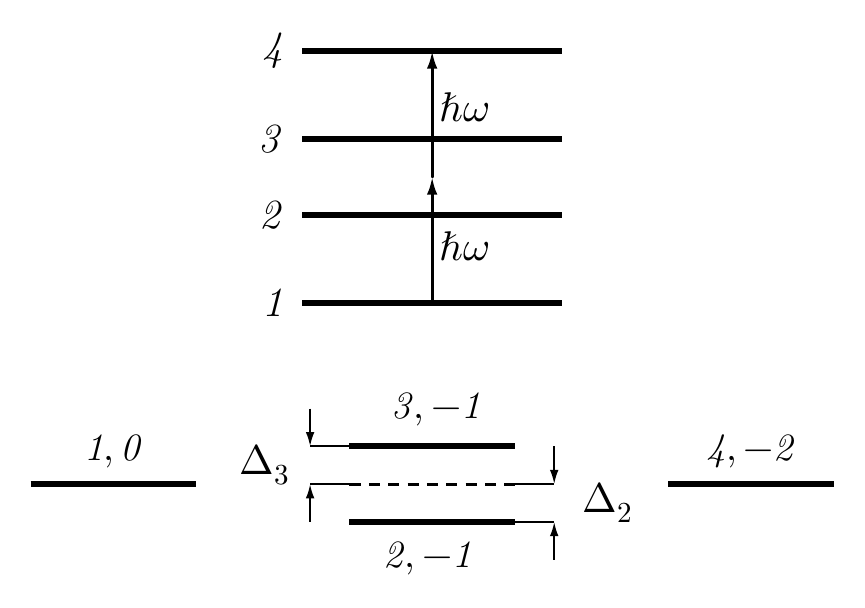
\begin{tikzpicture}[x=1cm,y=1cm]
\def\Es{1.60}\def\BaseUpper{3.60}\def\BaseLower{1.30}
\def\Eone{0}\def\Etwo{.7}\def\Ethree{1.3}\def\Efour{2}\def\Photon{1}
\foreach \n/\e in {1/\Eone,2/\Etwo,3/\Ethree,4/\Efour}{
 \pgfmathsetmacro\yy{\BaseUpper+\Es*\e}
 \coordinate (E\n) at (5.5,\yy);
 \draw[level] (3.85,\yy)--(7.15,\yy);
 \node[lab,anchor=east] at (3.68,\yy) {$\mathit{\n}$};}
\coordinate (Virtual) at (5.5,{\BaseUpper+\Es*\Photon});
% Exactly equal photon arrows: midpoint lies BETWEEN 2 and 3, not on either state.
\draw[photon] (E1)--node[lab,right,pos=.45] {$\hbar\omega$} (Virtual);
\draw[photon] (Virtual)--node[lab,right,pos=.55] {$\hbar\omega$} (E4);
\pgfmathsetmacro\yTwo{\BaseLower+\Es*(\Etwo-\Photon)}
\pgfmathsetmacro\yThree{\BaseLower+\Es*(\Ethree-\Photon)}
\pgfmathsetmacro\yFour{\BaseLower+\Es*(\Efour-2*\Photon)}
\draw[level] (.40,\BaseLower)--(2.50,\BaseLower);
\node[levlab,anchor=south] at (1.45,{\BaseLower+.13}) {$\mathit{1,0}$};
\draw[level] (4.45,\yTwo)--(6.55,\yTwo);
\node[levlab,anchor=north,fill=white,inner sep=1.6pt] at (5.44,{\yTwo-.19}) {$\mathit{2,-1}$};
\draw[level] (4.45,\yThree)--(6.55,\yThree);
\node[levlab,anchor=south,fill=white,inner sep=1.6pt] at (5.55,{\yThree+.20}) {$\mathit{3,-1}$};
\draw[level] (8.5,\yFour)--(10.6,\yFour);
\node[levlab,anchor=south] at (9.55,{\yFour+.13}) {$\mathit{4,-2}$};
\draw[virtual] (4.45,\BaseLower)--(6.55,\BaseLower);
% Delta3 upper, Delta2 lower, as in the authorial diagram.
\foreach \yy in {\BaseLower,\yThree}{\draw[baseline] (3.95,\yy)--(4.45,\yy);}
\draw[dim] (3.95,{\BaseLower-.48})--(3.95,\BaseLower);
\draw[dim] (3.95,{\yThree+.48})--(3.95,\yThree);
\node[lab,anchor=east] at (3.79,{.5*(\yThree+\BaseLower)}) {$\Delta_3$};
\foreach \yy in {\BaseLower,\yTwo}{\draw[baseline] (6.55,\yy)--(7.05,\yy);}
\draw[dim] (7.05,{\yTwo-.48})--(7.05,\yTwo);
\draw[dim] (7.05,{\BaseLower+.48})--(7.05,\BaseLower);
\node[lab,anchor=west,fill=white,inner sep=1.5pt] at (7.35,{.5*(\yTwo+\BaseLower)}) {$\Delta_2$};
\end{tikzpicture}

\end{document}
